\documentclass{article}
\usepackage{iclr2026_conference,times}
\usepackage[hidelinks,pdfstartview={}]{hyperref}
\usepackage{url}
\usepackage{booktabs}
\usepackage{amsmath,amssymb}
\usepackage{graphicx}
\usepackage{xcolor}
\usepackage{microtype}
\usepackage{enumitem}
\usepackage{makecell}
\usepackage[capitalise,noabbrev]{cleveref}
\setlist{itemsep=2pt,topsep=3pt}

\title{POST: Vision--Language Planners Use Stated\\Body Limits but Rarely Discover Them}

\usepackage[T1]{fontenc}
\iclrfinalcopy
\author{Yixuan Yang\\Independent researcher}
\begin{document}
\maketitle
\lhead{Preprint}

\begin{abstract}
A robot that plans with a vision--language model must choose tasks its own body can complete. We ask whether such a planner can obtain and use knowledge of its body. POST places an explicit body-rule layer over the AI2-THOR agent that varies one capability (mobility, reach or lifting capacity) between the two members of a pair, so that the correct choice of the heaviest deliverable object flips while the scene and candidates stay fixed. With a frozen Qwen3-VL-8B planner, stating the body profile and allowing reasoning yields 7 of 12 correct pairs (0 of 12 when an immediate answer is required), and watching a scripted self-checkup yields 9 of 12. Running its own checkup yields 1 of 12 with 12 action turns and 0 of 12 with 40. The saved traces show how the extra turns were spent: 540 of the 672 additional turns (80.4\%) are rotations or invalid turns. Under the same sufficient-evidence rule, only 2 of 24 self-run episodes reach sufficient evidence at either budget; all 24 watched checkups do, over 1,825 scripted actions. The planner can reason about body limits it is told or shown, but rarely gathers that evidence itself. The gap identifies self-testing policy as a distinct target for embodiment-aware planning.
\end{abstract}

\section{Introduction}

Language-model planners for robots must ground their plans in what the robot can actually do. SayCan combines a language model with learned affordance values for this purpose \citep{ahn2022saycan}, Inner Monologue feeds execution outcomes back into planning \citep{huang2022inner}, and a line of work in robotics builds self-models of a robot's own body \citep{cully2015robots,chen2022fullbody}. Recent embodied evaluation also identifies failures to track the body during navigation and interaction \citep{li2026humanclaw}. When a vision--language planner meets an unfamiliar body, a simpler question comes first: can it use body information if it has it, and can it get that information by testing itself?

POST (power-on self-test) isolates these two abilities. An agent with an unfamiliar body performs a self-test and then chooses the heaviest candidate object it can carry back to its dock. Pairs of episodes share the kitchen, the candidates and their stated masses, but differ in one body parameter, so that the correct choice differs between the members. As in answer-flipped question answering, a fixed preference (always the heaviest object, always the nearest) cannot solve a pair.

We compare five evidence-access conditions for one frozen planner: the body profile is stated (with an immediate or a reasoned choice), the planner runs its own checkup with 12 or 40 action turns, or the planner watches a scripted checkup while keeping notes. The result is a clear split (\cref{fig:results}). Told its profile and allowed to reason, the planner solves 7 of 12 pairs; watching an informative checkup, 9 of 12; testing itself, at most 1 of 12. Autonomous checkups rarely satisfy a sufficient-evidence rule, and a larger budget mostly bought rotations and invalid turns rather than evidence.

\paragraph{Contributions.} (i) A paired probe of embodiment awareness in which a single body parameter flips the correct task choice; (ii) evidence that a frozen VLM planner can use stated or observed body information but rarely acquires it through its own checkups; (iii) a trace-level evidence criterion, and a post-hoc count of feasibility-changing turns derived from it, that separate insufficient evidence from misuse of evidence, illustrated on a worked pair.

\section{The POST probe}

\paragraph{Task and body layer.} A body-rule layer over the default AI2-THOR agent \citep{kolve2017ai2thor} varies three capabilities: working drive motors (mobility), reach distance $\rho$ and lifting capacity $\mu$. This is an explicit rule-based task environment, not a physical robot or a learned dynamics model. The agent receives egocentric images and action outcomes, and may rotate, move, attempt a lift, put an object down, or finish testing. It must then choose the heaviest candidate that it can return to its dock; masses are stated.

\paragraph{Pairs and scoring.} The frozen benchmark has 12 pairs across seven kitchens, four for each body dimension. Pair members share the scene and candidate task but differ in one body parameter, so their correct choices differ. The primary score requires both choices in a pair to be correct. A script then attempts the selected delivery; this secondary outcome is not autonomous task planning and is not substituted for the choice score.

\paragraph{Conditions.} All conditions use one frozen Qwen3-VL-8B-Instruct model \citep{bai2025qwen3vl} with greedy decoding (\cref{tab:conditions}). Immediate choices allow 96 output tokens and reasoned choices 512; these response formats are part of the conditions, not an isolated token-budget manipulation. In checkup conditions, a four-entry window of recent observations and an editable NOTE carry information forward.

\begin{table}[t]
\centering
\caption{Evidence-access conditions in POST.}
\label{tab:conditions}
\small
\begin{tabular}{p{3.3cm}p{9.3cm}}
\toprule
Condition & What the planner receives \\
\midrule
Stated, immediate & Body parameters and dock distances; must choose immediately. \\
Stated, reasoned & The same information; may reason before the final JSON choice. \\
Own checkup, $K=12$ / $K=40$ & No profile. Up to $K$ action turns to test itself, then a reasoned choice. \\
Watched checkup & A frozen member-specific script is replayed while the planner records NOTE updates; then the same reasoned choice. \\
\bottomrule
\end{tabular}
\end{table}

The conditions differ in more than who selects the next action. Watched scripts execute 12--200 actions (about 76 on average; 1,825 in total, against 288 and 960 action turns for the two autonomous budgets), request NOTE updates at selected outcome-bearing events, and can restore an object's pose after a successful put-down. The stated profile also supplies dock distances that an autonomous agent must acquire. These are relevant advantages, so the comparisons are diagnostic rather than a budget- and information-matched planning ablation.

\paragraph{Evidence criterion.} To separate missing evidence from misused evidence, a frozen sufficient-evidence rule checks whether an episode's logged outcomes determine a unique feasible choice. The rule certifies a candidate feasible after a successful lift, and infeasible after a lift-limit failure or after a reach failure in an episode where disabled motors have been observed; a motor failure can therefore certify an earlier reach failure.

\paragraph{Feasibility-changing turns (post hoc).} To ask whether longer checkups at least gather more task-relevant evidence, we replay the unchanged rule over every logged action prefix of the existing trajectories and count a turn when the candidates' feasible/infeasible mapping after it differs from the mapping before it. A turn that certifies several candidates counts once; invalid turns, a motor failure that certifies nothing, and a new heading without a feasibility change do not count. The count measures progress toward this task's existing certificate, not all visual or body information an observation may carry. The replay reproduces the original sufficient-evidence counts.

\section{Results}

\begin{table}[t]
\centering
\caption{\textbf{Stated or watched body evidence is used; self-gathered evidence is rare.} Evidence counts apply the frozen sufficient-evidence rule to checkup traces. Delivery is a secondary scripted endpoint; the $K=40$ delivery count is not reported.}
\label{tab:results}
\begin{tabular}{lcccc}
\toprule
Condition & Pairs /12 & Choices /24 & Evidence /24 & Delivery /24 \\
\midrule
Stated, immediate & 0 & 12 & -- & 9 \\
Stated, reasoned & 7 & 19 & -- & 11 \\
Own checkup, $K=12$ & 1 & 9 & 2 & 6 \\
Own checkup, $K=40$ & 0 & 9 & 2 & -- \\
Watched checkup & 9 & 21 & 24 & 10 \\
\bottomrule
\end{tabular}
\end{table}

\begin{figure}[t]
\centering
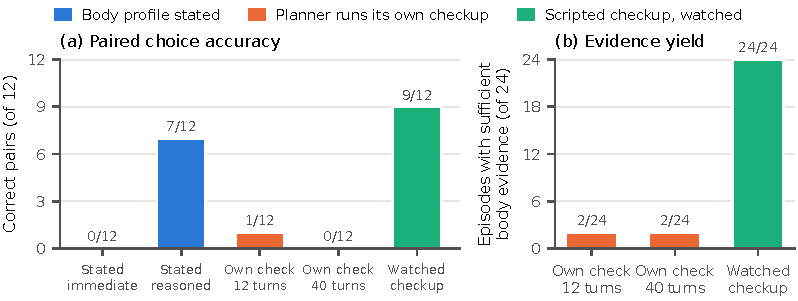
\includegraphics[width=\linewidth]{figures/post_fig_results.pdf}
\caption{\textbf{The planner chooses well when told or shown its limits, and poorly when it must test itself.} (a) Correct pairs out of 12. (b) Checkup episodes whose logged outcomes satisfy the sufficient-evidence rule.}
\label{fig:results}
\end{figure}

\paragraph{The reasoned response format improves use of stated information.} With the profile stated, an immediate choice solves no pair, while a reasoned choice (with a larger output allowance, 512 rather than 96 tokens) solves 7 of 12 pairs and 19 of 24 member choices (\cref{tab:results}). The planner can combine stated masses, reach, mobility and dock distances into a feasible choice when the response format allows reasoning.

\paragraph{Watching a checkup works; running one rarely does.} Watched checkups reach 9 of 12 pairs and 21 of 24 choices. Autonomous checkups reach 1 of 12 pairs with 12 turns and 0 of 12 with 40, with nine correct member choices in both. A model can therefore make substantially better conditional choices when supplied with information than after its own tested checkup.

\paragraph{Autonomous checkups rarely yield sufficient evidence.} Only two autonomous episodes at $K=12$ satisfy the sufficient-evidence rule, and both choose correctly. At $K=40$ the evidence yield stays at two despite the larger budget; that run contains 190 invalid turns and much rotation. Watched scripts satisfy the rule in all 24 episodes, with 21 matching choices. When an episode satisfies the rule, the planner usually chooses correctly; its own checkups rarely get there.

\paragraph{More turns bought rotations, not evidence.} An optimistic static audit on saved reachable grids shows that 14--19 actions are needed for sufficient evidence in the eight lift-limit episodes, ignoring visibility, holding, put-down and return costs, so 12 turns are restrictive for that criterion. The 40-turn run tests that explanation, and \cref{tab:actions} shows how the extra turns were spent. Of the 672 additional action turns, 540 (80.4\%) are additional rotations (364) or invalid turns (176). Lift attempts rise from 62 to 96 (2.58 to 4.00 per episode), yet feasibility-changing turns stay flat (20 at 12 turns, 19 at 40); under both budgets 12 of 24 episodes gain at least one candidate-feasibility fact and 2 reach sufficient evidence. The watched scripts yield 72 feasibility-changing turns and sufficient evidence in all 24 episodes over 1,825 scripted actions. The differing budgets and information access are described in the conditions above.

\begin{table}[t]
\centering
\caption{\textbf{A larger budget adds rotations and invalid turns, not feasibility evidence.} Action mix and post-hoc feasibility-changing turns over the 24 checkup episodes of each condition. Changes: turns that change the certified feasibility of any candidate. Members: episodes with at least one such turn. Sufficient: episodes whose final evidence satisfies the rule.}
\label{tab:actions}
\small
\setlength{\tabcolsep}{3.4pt}
\begin{tabular}{lrrrrrrrrr}
\toprule
Condition & Rotate & Move & \makecell{Lift\\attempts} & \makecell{Put\\down} & Invalid & \makecell{Action\\turns} & Changes & Members & Sufficient \\
\midrule
Own checkup, $K=12$ & 131 & 66 & 62 & 15 & 14 & 288 & 20 & 12 & 2 \\
Own checkup, $K=40$ & 495 & 159 & 96 & 20 & 190 & 960 & 19 & 12 & 2 \\
Watched checkup & 360 & 1,305 & 100 & 60 & 0 & 1,825 & 72 & 24 & 24 \\
\bottomrule
\end{tabular}
\end{table}

\begin{figure}[t]
\centering
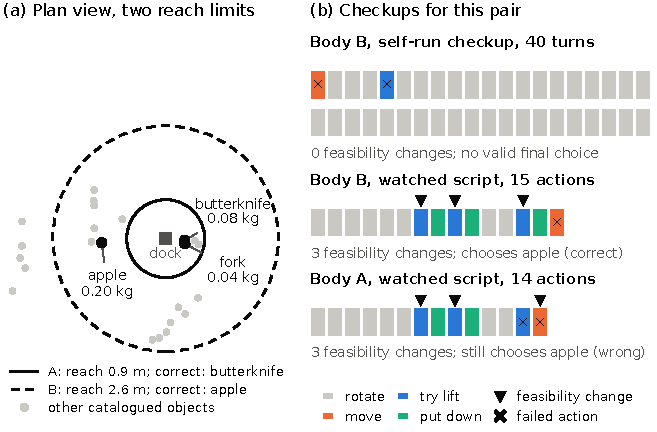
\includegraphics[width=\linewidth]{figures/post_fig_reach.pdf}
\caption{\textbf{More testing turns need not produce task-relevant evidence, and sufficient evidence need not be used.} A recorded reach pair (FloorPlan6), selected to illustrate the 40-turn rotation loop. (a) Plan view from the logged $x$--$z$ coordinates of the saved scene catalogue; circles show the nominal reach radii, while the recorded dock distances also include a small vertical component. (b) Logged action sequences. Body B's 40-turn self-run contains 38 rotations, no feasibility change and no valid final choice. Its watched script certifies all three candidates with lifts at actions 7, 9 and 13, and the planner chooses the apple. Body A's watched script certifies the butterknife as the heaviest feasible candidate, but the planner still chooses the apple.}
\label{fig:reach}
\end{figure}

\paragraph{A worked pair.} \Cref{fig:reach} follows one reach pair, chosen to illustrate the 40-turn rotation loop in a task whose body change is easy to explain. Both bodies have disabled drive motors and a 10\,kg lift limit; body A reaches 0.9\,m and body B 2.6\,m. The candidates are a fork (0.04\,kg, recorded dock distance 0.456\,m), a butterknife (0.08\,kg, 0.441\,m) and an apple (0.20\,kg, 1.480\,m), so the correct choice is the butterknife for A and the apple for B. In its 40-turn self-run, body B rotates 38 times, attempts one move, which fails on the disabled motors, and one lift of the fork, which fails because the fork is not in view; no turn changes a candidate's feasibility, and the planner gives no valid final choice. Its watched script takes 15 actions: successful lifts at actions 7, 9 and 13 certify all three candidates feasible, and the planner correctly chooses the apple. Body A's watched script takes 14 actions: the fork and butterknife lift, the apple lift fails on reach, and a final motor failure certifies the apple infeasible, so the evidence supports the butterknife; the planner still chooses the apple, making this one of the three watched episodes whose sufficient evidence did not produce a matching choice. No checkup condition solves this pair. In the 12-turn self-run and in the watched condition the planner chooses the apple for both bodies, the choice a fixed preference for the heaviest object would make; at 40 turns body A chooses the butterknife correctly and body B gives no valid choice. With the profile stated, the immediate choice is the apple for both bodies, wrong for A. The reasoned choice is correct for both: body A rejects the apple as out of reach and takes the heavier reachable utensil, and body B takes the apple, although its stated rationale (``I can walk to it'') ignores the disabled motors. A correct choice is also not a completed delivery: the scripted delivery of A's butterknife fails because the knife is not in view from the starting heading, whereas B's apple is delivered in both stated variants.

\section{Discussion and next steps}
POST shows two separable deficits in a frozen VLM planner. The first is a response-format effect: the stated profile yields 7 of 12 correct pairs with the reasoned response protocol and none with an immediate choice. The second is an acquisition failure: the planner's own checkups rarely produce evidence that satisfies the rule, and a larger budget produced no additional qualifying episodes in this run (the 40-turn run contains 190 invalid turns). Both mirror findings on evidence about the world in the companion EPACT benchmark \citep{yang2026epact}, where models answer from supplied views but rarely obtain those views themselves, and where policies often repeat an observation action whose result they have already seen; the 40-turn rotation loop is a similar repetition in a self-test, here before any feasibility evidence has been gathered. The worked pair adds a third, smaller deficit: sufficient evidence is not always used. Together, these results motivate training self-test policies to select actions that resolve task feasibility, while retaining a separate check on whether the planner uses the evidence they obtain.

\section{Related work}
\paragraph{Grounding plans in capabilities.} SayCan scores language-model proposals with learned affordance values \citep{ahn2022saycan}, and Inner Monologue feeds environment feedback back into planning \citep{huang2022inner}. Physically grounded VLMs fine-tune on physical-property annotations such as mass and fragility \citep{gao2024physically}. POST asks whether a frozen VLM planner can infer and use constraints of its own body rather than properties of objects.

\paragraph{Self-models.} Robots that adapt like animals build and exploit models of their own behavior after damage \citep{cully2015robots}, and visual self-modeling learns a robot's morphology from its own observations \citep{chen2022fullbody}. HumanCLAW separates high-level action decisions from low-level motor execution and measures body-awareness failures during navigation and interaction \citep{li2026humanclaw}. POST instead holds the scene and candidates fixed while changing one explicit capability, and compares whether a planner uses stated or observed limits with whether it discovers them through self-tests.

\paragraph{Active perception and embodied QA.} POST's checkups are active perception directed at the agent itself \citep{bajcsy1988active,bohg2017interactive}; its paired scoring follows the answer-flipped design of the companion EPACT benchmark \citep{yang2026epact}, in the lineage of \citet{das2018embodied} and \citet{majumdar2024openeqa}.

\section{Limitations}
POST's 12 pairs do not cover physical embodiment broadly; its rule layer abstracts dynamics; one model is evaluated with greedy decoding; watched scripts are not budget-matched; profile disclosure changes the available information; and delivery is scripted. The paired score removes fixed-prior success but does not guarantee the intended reasoning path. Results are descriptive counts, and no training or multi-seed adaptation is claimed. The feasibility-change count is a post-hoc diagnostic under one formal rule, the watched reference uses a different action budget, and the worked pair was selected for illustration.

\section{Conclusion}
The tested frozen vision--language planner uses body limits it is told or shown but rarely discovers them by testing itself, and a larger testing budget mostly bought rotations and invalid turns rather than evidence. Paired body-flipped choices make this gap visible with a handful of episodes, and give a target for training planners that test themselves before they commit.

\section*{Data and code availability}
Companion method code, frozen pairs, checkup traces and score-replay scripts are included as ancillary files. Their scope is described in \cref{app:repro}.

\bibliography{references}
\bibliographystyle{iclr2026_conference}

\appendix
\section{Reproducibility}
\label{app:repro}
The companion materials, included as ancillary files with this preprint, provide the body-rule layer, frozen pairs and checkup scripts, compact scoring records and analysis code. A CPU replay recomputes the reported scores and applies the unchanged sufficient-evidence rule to every action prefix in all 72 checkup episodes; it reproduces the original sufficient-evidence counts. The public choices are the preserved parser outputs, not a new parsing of undistributed model replies. \Cref{fig:reach} is drawn from the logged coordinates of the saved scene catalogue and the exact logged action sequences. Model weights and upstream simulator assets are obtained separately, and relocated model and simulator execution has not been rerun. Code is released under the MIT license; third-party terms remain applicable.

\end{document}
